\documentclass{article}
\usepackage{tikz}
\usepackage{tikz-qtree}
\begin{document}
\tikzset{edge from parent/.append style={->}}
\tikzset{every tree node/.style={draw}}

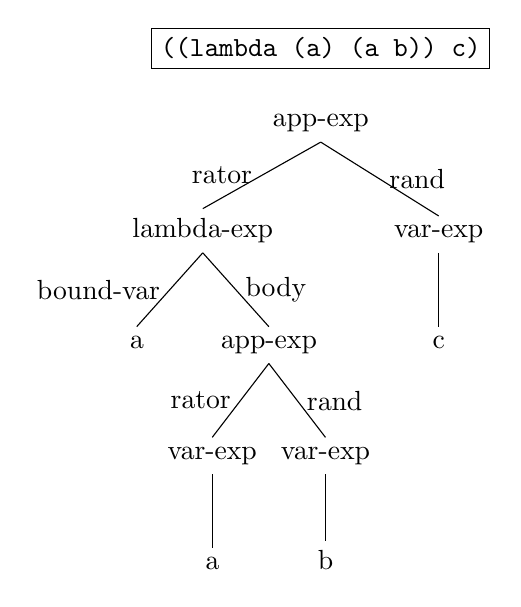
\begin{tikzpicture}[level distance=40pt]
  \node[rectangle,draw] {\verb|((lambda (a) (a b)) c)|};
  \begin{scope}[yshift=-1cm]
    \Tree [.app-exp
      \edge node[midway,left]{rator};
      [.lambda-exp
        \edge node[midway,left]{bound-var}; a
        \edge node[midway,right]{body};
        [.app-exp
          \edge node[midway,left]{rator}; [.var-exp a ]
          \edge node[midway,right]{rand}; [.var-exp b ] ] ]
      \edge node[midway,right]{rand}; [.var-exp c ] ]
  \end{scope}
\end{tikzpicture}
\\[1cm]
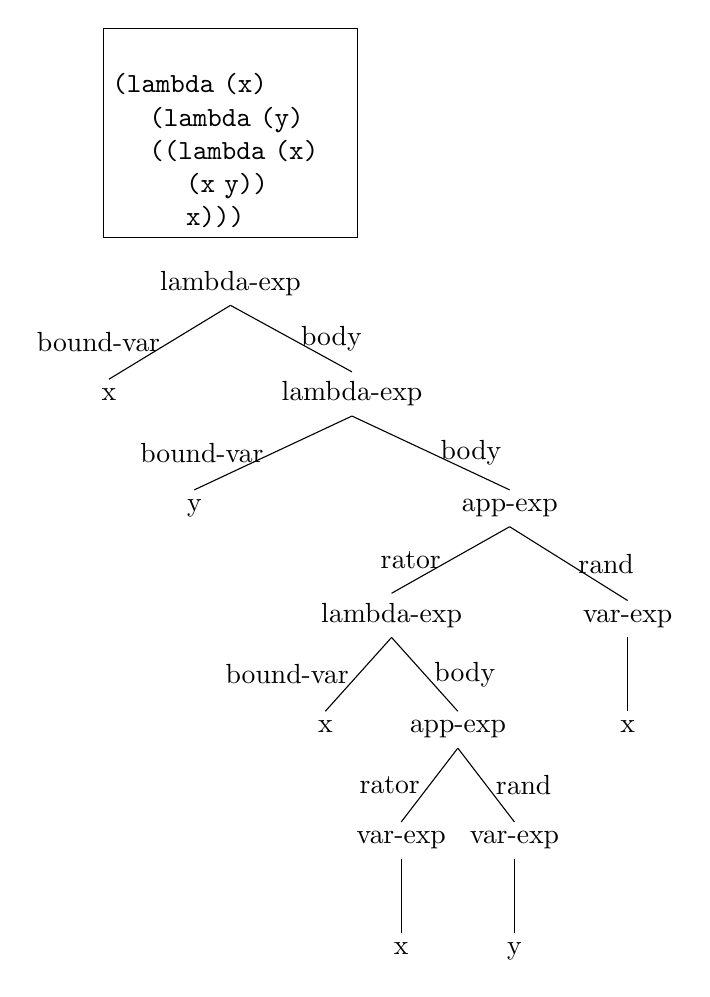
\begin{tikzpicture}[level distance=40pt]
  \node[rectangle,draw] [text width=3cm]{\begin{verbatim}
(lambda (x)
    (lambda (y)
    ((lambda (x)
        (x y))
        x)))
\end{verbatim}
  };
  \begin{scope}[yshift=-2cm]
    \Tree [.lambda-exp
      \edge node[midway,left]{bound-var}; x
      \edge node[midway,right]{body};
      [.lambda-exp
        \edge node[midway,left]{bound-var}; y
        \edge node[midway,right]{body};
        [.app-exp
          \edge node[midway,left]{rator};
          [.lambda-exp
            \edge node[midway,left]{bound-var}; x
            \edge node[midway,right]{body};
            [.app-exp
              \edge node[midway,left]{rator}; [.var-exp x ]
              \edge node[midway,right]{rand}; [.var-exp y ] ] ]
          \edge node[midway,right]{rand}; [.var-exp x ] ] ] ]
  \end{scope}
\end{tikzpicture}
\end{document}
